\section{Introduction system environment}
\label{ch:practical_realization:sys_env}

Containerization has been successfully established in Linux environments.
However it is also available in other environments like Windows and MacOS.
Containerization via Docker in Windows and MacOS is implemented through the use of an emulated Linux underneath.
The prototype will be developed for a pure Linux environment since basic concepts are available natively under Linux as known from the background chapter.
The well known and stable system Debian GNU/Linux is used as a derivative. 
Other Linux major distributions like the SUSE or RedHat family are not considered directly. 
The reason for the Debian based system is the already gained knowledge about Debian systems in the past. 

The landscape of the system environment including working environment is shown in Figure \ref{fig:pract:sys_env}.
\begin{figure}[h!]
 \centering
 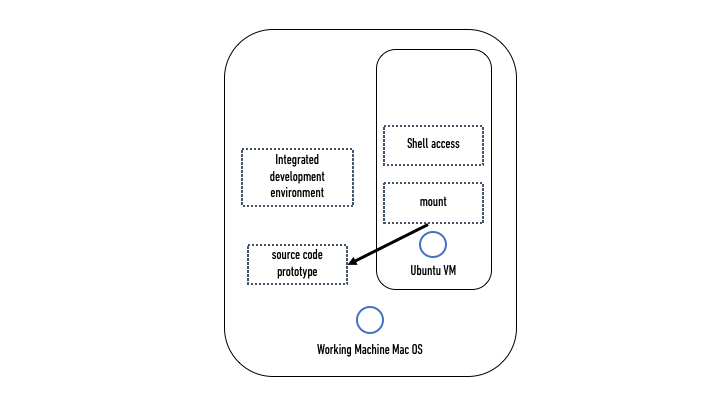
\includegraphics[width=0.8\textwidth]{gfx/examples/sys_env.png}
 \caption{Local development environment}
 \label{fig:pract:sys_env}
\end{figure}
The MacOS working machine locally provides a headless Ubuntu as a virtual machine. 
The hypervisor is the well known VirtualBox.
The code itself is written on the working machine and mounted on the virtual machine. 
This allows code accessing and execution on the virtual machine through a ssh tunnel. 
This corresponds to the idea that the prototyp is operated and tested on a simple Linux system.

Python is used as programming language for this prototyp. 
The decision of using Python can be made very uncomplicated in this context. 
A very useful Python library for the Docker API is existing. 
This API allows everything the Docker command does. 
This includes starting, stopping and altering of containers and images amongst other resources. 
All available actions can be viewed in the official documentations \cite{python_sdk}. 

Python is an interpreted programming language that allows to run the same code on multiple platforms without recompilation. 
Hence it is not required to recompile the code after making any alteration. 
This interpreting mechanism makes programming and testing easier and faster during the development process.

Furthermore Python provides an easy syntax which is readable by any english speaker. 
For those developers who are not familiar with Python it is like reading pseudo code. 
This makes it easier to adapt this prototyp in a larger project with a different technology stack.

Lastly Python provides a helpful module called virtual environment (venv). 
Virtual environments create a dedicated Python environment that allows packages to be installed, modified and used without disturbing the global Python binary. 
This feature is used to manage the necessary packages like for instance the Docker SDK. 
This feature is especially useful when the tool is delivered to a remote system. 
The tool works independent in existing Python instances. 
In this context it is worth to know that Python in version 2.x has not been supported anymore since January 2020 \cite{python_deprecated}. 
Accordingly the newest supported long term Python version is used. 
The same applies to the Python package manager Pip. 
The package manager should correspond to Python in a compatible version. 
The exact versions of this prototyp is Python 3.7 and Pip3.

Now the system environment and the programming language to be used is well defined. 
With this in mind the next section shows the general project structure of the prototyp.